\documentclass{article}
\usepackage{amsmath}
\usepackage{graphicx}

\title{Lecture 2}
\author{Dark Lord}

\begin{document}
\maketitle

\section*{Equations}


\begin{equation}
    \label{limit}
    e = \lim_{t \to \infty} {\left( 1+t \right)}^t
\end{equation}


\begin{align}
    % \label{limit2}
    e  &= \lim_{t \to \infty} {\left( 1+t \right)}^t\\
    \text{Like and Subscribe} &= \lim_{t \to \infty} {\left( 1+t \right)}^t
\end{align}

\begin{equation}
\begin{split}
    % \label{limit3}
    e &= \lim_{t \to \infty} {\left( 1+t \right)}^t \\
    \text{Like and Subscribe} &= \lim_{t \to \infty} {\left( 1+t \right)}^t
\end{split}
\end{equation}
% Equation 1 is very cool
Equation~\ref{limit} is very cool


 % for long equations which do not fit in one line

\begin{multline}
    e \approx 1+x+ \frac{x^2}{2!}+ \frac{x^3}{3!} + \frac{x^4}{4!} + \frac{x^5}{5!}\\    
    +\frac{x^6}{6!} + \frac{x^7}{7!} + \frac{x^8}{8!}
\end{multline}


\newpage

\section{Tables}



\begin{table}
\caption{NIFTY table}\label{niftytable}
\begin{center}
    \begin{tabular}{|c|r|}
        \hline
        1 & 2 \\ \hline
        3 & 400000000000000 \\ \hline
    \end{tabular}
\end{center}
\end{table}

I like table no~\ref{niftytable}

\begin{figure}
    \centering
    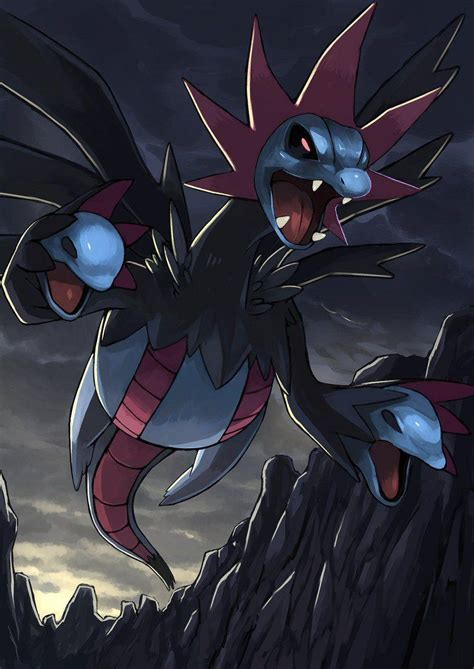
\includegraphics[width=\textwidth]{img1}
    \caption{Hydreigon}\label{hydreigon}



\end{figure}

\end{document}
